Les objectifs de ce troisième hands-on sont:
\begin{itemize}
	\item[-] D'introduire le concept de distorsion d'un signal, en particulier la notion d'overdrive/clipping.
	\item[-] De comprendre le fonctionnement et d'implémenter un circuit généralement utilisé pour des pédales de guitare électrique, permettant de générer un effet d'overdrive sur le signal sonore.
\end{itemize}
\vspace{.25cm}

\begin{figure} [!ht]
	\centering
	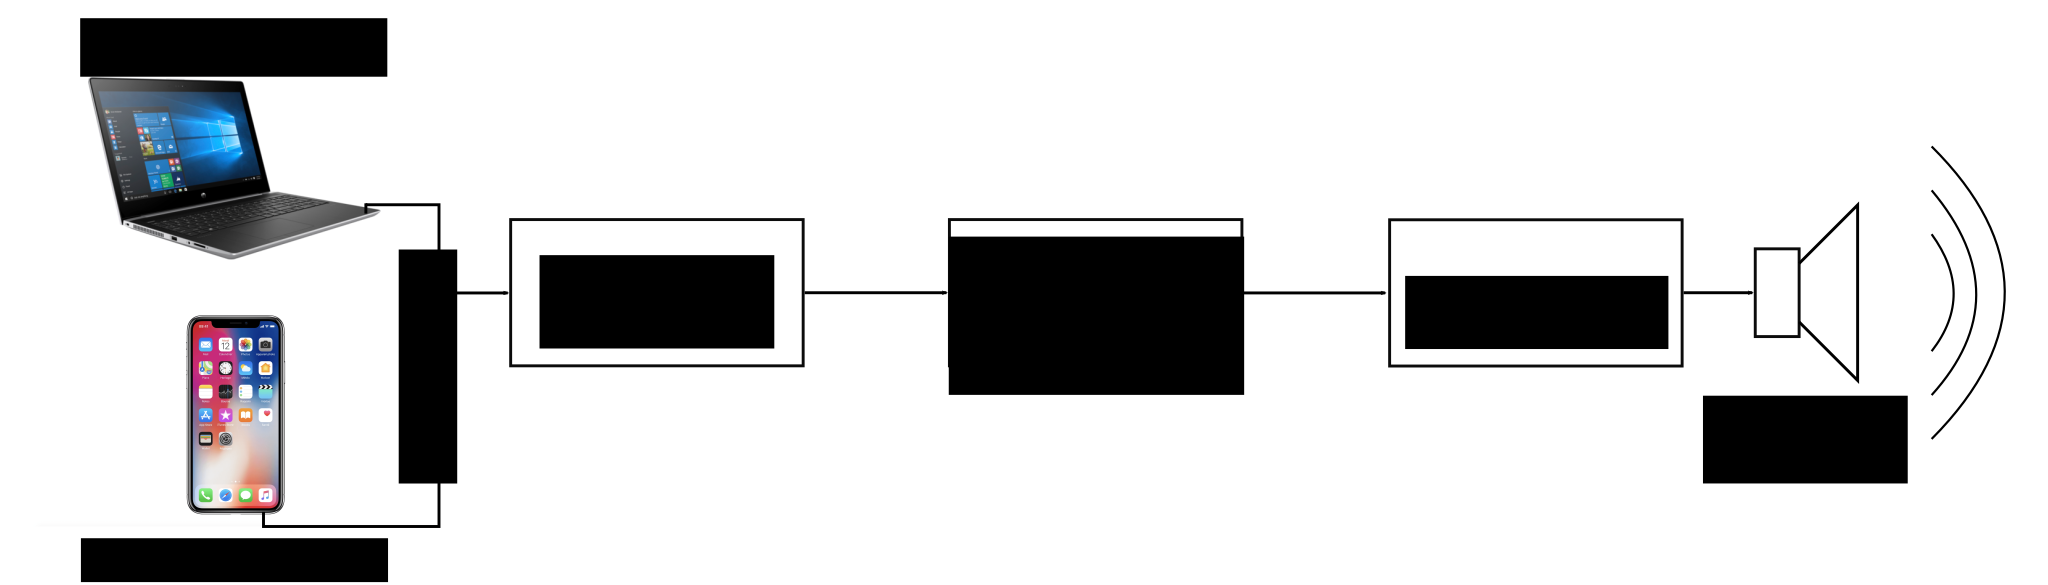
\includegraphics[width=.95\textwidth]{block-diagram}
	\caption{Schéma-bloc du circuit, avec ajout du bloc de distorsion.}
	\label{fig1:block-diagram}
\end{figure}

Le schéma-bloc du circuit modifié est présenté à la Figure \ref{fig1:block-diagram}. En comparaison avec la version proposée lors du second hands-on, on constate maintenant la présence d'un bloc de distorsion entre le bloc de filtrage et l'amplification. Par ailleurs, le contrôle du volume a été déplacé en sortie du bloc de distorsion. Ce bloc va permettre de clipper le signal sonore filtré et ainsi de produire l'effet d'overdrive caractéristique des sons de guitare électrique.